\chapter{Integrating structural feedback in conceptual design tools}
\label{ch:Integrating structural feedback}
In the conventional workflow the architect uses geometric modelling tools and the engineer deploys structural analysis tools in a sequential step. Parametric modeling tools are an improvement to this workflow, as structural analysis plug-ins are available. This allows the user to get structural feedback earlier in the design phase, but still as a sequential step to the geometric modeling.

The present work purposes an improvement to the workflow by integrating structural feedback with geometric modeling. However, this creates new demands on conceptual design tools. 

\section{Human-computer interaction}
The conceptual design tools should inspire and encourage the user to explore design alternatives. This puts demands on the human-computer interaction of such tools. The tools need to be interactive and allow the user to, quickly create new models, or to make changes to existing models. 

Direct manipulation is a human-computer interaction style that enables the user to directly manipulate objects on the screen, and by doing so, reducing the perceptual and cognitive resources required to understand and use the user interface. In Paper 1, a conceptual design tool has been created which employs a very direct manipulation user interface for 2D. This is achieved by taking advantage of the multi-touch screen – which literally closes the gap between human and computer. In this work, the user can input a structural model by using gestures similar to those found in drawing applications for tablets, see Figure \ref{fig:interaction}. This allows the user to quickly explore different design alternatives.

\begin{figure}
  \includegraphics[width=330pt]{graphics/interaction.eps}
  \caption{Modelling gestures in the developed application Sketch a Frame}
  \label{fig:interaction}
\end{figure}

Achieving a very direct manipulation in 3D is today possible with the emergence of new 3D input controllers. This creates an opportunity to create conceptual design tools with a very direct manipulation for 3D. In Paper B, this opportunity has been explored by developing a conceptual design tools which employs a very direct manipulation for 3D. This has been achieved by using a 3D input controller named the Leap Motion Controller. 

In Paper A, a very direct manipulation cycle is purposed which further improves interactivity of the user interface of conceptual design application. As the user is modelling, computations are continuously performed, and when the modeled structure is stable the result is automatically visualized. This removes the need for a specific “compute step” which further integrate structural feedback into the geometric modelling. This direct manipulation cycle is also employed in the developed application in Paper B.

\section{Structural feedback}
To integrate structural feedback into conceptual design applications structural analysis must be integrated with the geometrical modeling. The feedback should also be easy to understand and provide valuable feedback of the structural behavior and performance.

\begin{figure}
  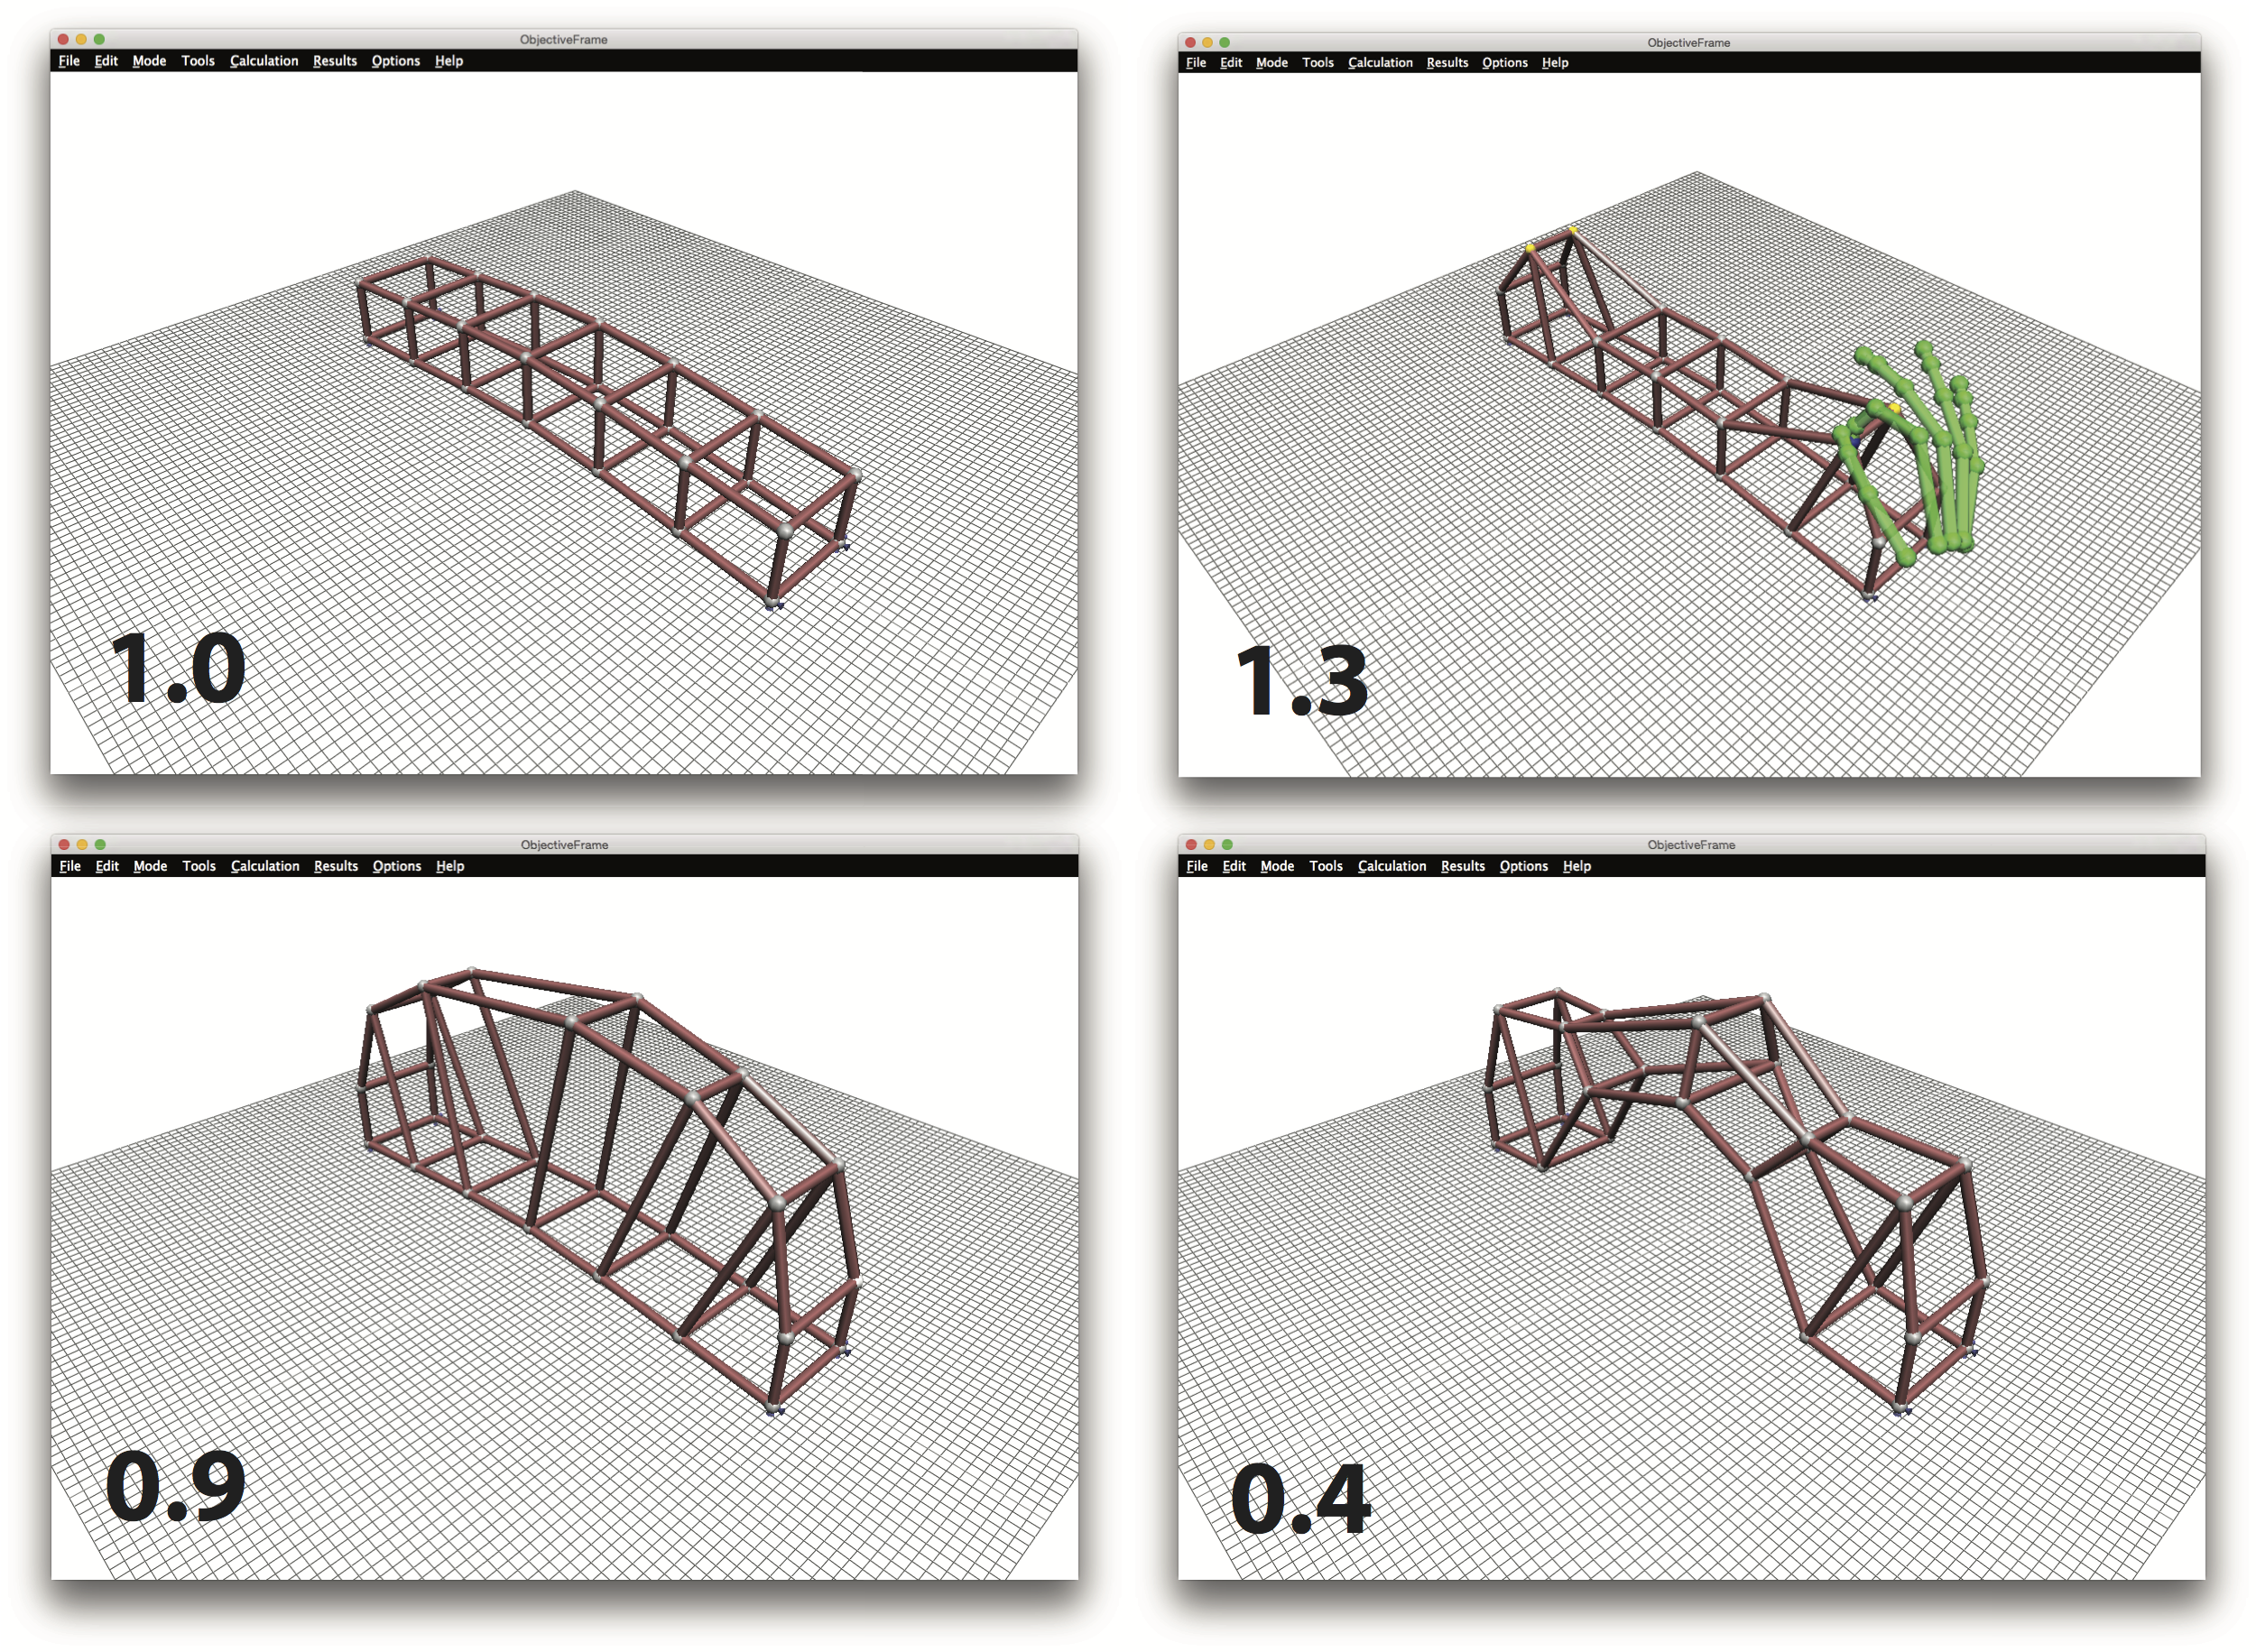
\includegraphics[width=350pt]{graphics/performance-feedback.png}
  \caption{Geometric modeling with real-time performance index}
  \label{fig:performance-feedback}
\end{figure}

In the developed applications in Paper A and Paper B, an external force can be applied to the modeled structure. If the model is stable – the resulting deformations can be visualized in real-time. The user can then manipulate the force using direct manipulation, and in real-time see how the structural deformation responds. In Paper A, when an external force has been applied, the resulting normal forces and the moment envelope can also be visualized in real-time. This can improve the user’s understanding of, how the structure responds to external forces - how stresses follow through the different members, and the stiffness of the structure in different directions.

The structural feedback should be easy to understand for the user. In Paper B, a model can be manipulated by the previously described direct manipulation methods, simultaneously the user is presented with a performance index, which is a measure of how well performing the structure is. The performance index is the normalized strain energy of the model; thus a lower number means a better performing structure, see Figure \ref{fig:performance-feedback}. Presenting a single number that represents how well performing the structure is makes it easy for the user to understand how geometrical modifications affects the structural performance.


\section{Structural optimization}
Integrating structural optimization into conceptual structural design has the possibility to not only give feedback of the structural performance but also to guide the user towards geometries that are structurally well performing. 

A genetic algorithm has been implemented in the application described in Paper A, which can be used for shape optimization. The user first selects which nodes and in which direction (vertical or horizontal) that the optimizer is allowed to move the nodes. Then the optimization can be executed and the strain energy is minimized. After the analysis is complete the best performing structure is visualized, see Figure \ref{fig:ipad-ga}. 

\begin{figure}
  \includegraphics[width=330pt]{graphics/ipad-ga.png}
  \caption{Genetic algorithm optimization in Sketch a Frame}
  \label{fig:ipad-ga}
\end{figure}

Form finding can be used to find the static equilibrium for a structure under load. In Paper B, the dynamic relaxation method has been implemented to enable form finding in an interactive 3D environment. The user can further explore the form found structure by applying and manipulating an external force. The point load can here be used to move away from the optimal solution in order to find other interesting sub optimal solutions that might be more aesthetically attractive to the user. The point load can also, for example, represent a supporting column or a hanging installation in the structure.


\section{Visual representations}
After structural analysis computations have been performed the result can be visualized. For conceptual structural design tools, visualization where the user can quickly get an understanding of the results are sought. 

One such example is graphic statics, which visualize forces as lengths of lines in the force diagram. This is beneficial for the users understanding, compared to using colors to represent the size of the forces, as it removes a layer of abstraction. The user can directly understand the size of the forces without the need of a for example a colorbar.

To visualize dynamic behavior animations can be used. This is used in the application developed in Paper A – if a force is applied to a non-stable model the corresponding mechanism is visualized by using an animation. This allows the user to quickly understand the model’s non-stable behavior, and how the model needs to be modified in order to make it stable. 

\subsection{Example - Loadpaths}
Structural behavior of 1D elements, such as bar and beam elements, are easier to understand than higher dimensional elements. Higher dimensional elements have a more complex structural behavior. For 2D structural elements the internal stresses can be computed and used to compute lines which represents how the external load flows through the structure towards the boundary conditions. Here described for the Z-direction \cite{Fonseca1997}:

\begin{equation*}
\frac{\delta \tau_{xz}}{\delta x} + \frac{\delta \tau_{yz}}{\delta y} + \frac{\delta \sigma_{z}}{\delta z}= 0
\end{equation*}

The author has explored how loadpaths can be extended into 3D by using volumetric elements. The idea for the algorithm and the result is shown in Figure \ref{fig:flowlines-exp}. Volumetric elements are colored according to the von Mises stress and the green dots are boundary conditions. However, this method does have some drawbacks; it is unclear how to interpret the lines, sensitivity to the mesh and computational heavy. Also, only the internal stresses acting in the Z-direction are here considered.
 
\begin{figure}
  \includegraphics[width=330pt]{graphics/flowlines-exp.eps}
  \caption{Computing loadpaths for 3D}
  \label{fig:flowlines-exp}
\end{figure}